\documentclass{note}
\usepackage{mypackage}

\renewcommand{\thefootnote}{\fnsymbol{footnote}}

\title{数字电路与逻辑设计笔记}
\author{陈鸿峥}
\date{{\builddatemonth\today} \footnote{\text{Build \builddate\today}}}%加了build

\begin{document}

\maketitle
\renewcommand{\thefootnote}{\arabic{footnote}}
\setcounter{footnote}{0}

\setcounter{tocdepth}{2}%设置深度
\tableofcontents

% !TEX root = main.tex

\section{计算机系统概述}
\subsection{计算模型}
\begin{itemize}
	\item 图灵机(1936)
	\item 冯诺依曼体系结构(1945)\footnote{非冯诺依曼体系结构:并行计算、量子计算、生物计算} --- 存储程序原理(\textbf{运算器}为中心)\\
	计算机采用\textbf{二进制}表示机器指令和数据,按照程序指令\textbf{顺序}执行
\begin{center}
\begin{tikzcd}
& & \text{存储器}\arrow{d} & & \\
\quad\arrow{r} & \text{输入设备}\arrow{r} & \text{运算器}\arrow{r}\arrow{d}\arrow{u} & \text{输出设备}\arrow{r} & \quad\\
& & \text{控制器}\arrow{u}\arrow{lu}\arrow{ru}\arrow[bend left]{uu} & &
\end{tikzcd}
\end{center}
而现在由于计算不是瓶颈,存储访问成为了瓶颈,故现代微机以\textbf{存储器}为中心
\begin{center}
\begin{tikzcd}
& & \text{运算器}\arrow{d} & & \\
\quad\arrow{r} & \text{输入设备}\arrow{r} & \text{存储器}\arrow{r}\arrow{d}\arrow{u} & \text{输出设备}\arrow{r} & \quad\\
& & \text{控制器}\arrow{u}\arrow{lu}\arrow{ru}\arrow[bend left]{uu} & &
\end{tikzcd}
\end{center}
\end{itemize}
[运算器、控制器](CPU)、存储器为计算机的核心,合称主机;外围设备,简称外设,指除主机外的其他设备,包括IO设备、外存等

计算机中的信息仍用二进制表示的原因:由物理器件性能决定
\begin{itemize}
	\item 二进制只有两种状态,容易找到具有2个稳定状态并且状态转换容易控制的物理器件(数字电路)
	\item 二进制编码运算规则简单
	\item 二进制的0、1与二值逻辑一致,容易实现逻辑运算
\end{itemize}
% There are two reasons computers use the binary system:
% 1.Two clearly distinct states that provide a safety range for reliability.
% 2.Least amount of necessary circuitry, which results in the least amount of space, energy consumption, and cost.

\subsection{计算机的发展历程}
按发展历程可分为:电子管、晶体管、集成电路、(超)大规模集成电路四代计算机
\par重大历史事件如下
\begin{center}
\begin{tabular}{|c|c|c|c|}
\hline
% 年份 & 姓名 & 事件 & 备注 \\
1904 & 弗莱明(Fleming) & 二极管 & \\\hline
1907 & 德福雷斯特(De Forest) & 三极管 & \\\hline
1938 & 香农(Shannon) & 布尔代数与二值电子器件(继电器) & 奠定数字电路基石 \\\hline
1946 & & 第一台通用计算机ENIAC & 十进制 \\\hline
1947 & \begin{tabular}{c}布莱顿(Brattain)\\
巴丁(Bardeen)\end{tabular} & 点接触晶体管 & \\\hline
1949 & 肖克利(Shockley) & 结型晶体管(1949) & 1956诺贝尔奖\\\hline
1950 & & 二进制和存储程序EDVAC & 实现冯诺依曼设想(组合进步) \\\hline
1958 & Jack Kilby & 集成电路 & 2000诺贝尔奖 \\\hline
1965 & Moore & 摩尔定律 & \begin{tabular}{c}
在价格不变的情况下,每18个月芯片上\\
晶体管数目翻倍,性能也提升一倍
\end{tabular}\\\hline
1971 & Intel & 第一款微处理器4004 & 10$\mu$m\\\hline
\end{tabular}
\end{center}

\subsubsection{单处理器(1971-2002)}
性能提升主要手段
\begin{itemize}
	\item 提升工作主频:KHz增长至GHz(生产工艺进步,流水线级数增加)
	\item 指令级并行(ILP)
\end{itemize}
\begin{proposition}[安迪-比尔定律]
Andy gives, Bill takes away. 安迪是原Intel CEO,比尔是原微软CEO,硬件厂商靠软件开发商用光自己提供的硬件资源得以生存
\end{proposition}
但遇到频率墙和功耗墙
\[\text{功耗(power)}\propto 1/2\times\text{CMOS电容}\times\text{电压}^2\times\text{转换(01)频率}\]
\par
2004年,Intel放弃4GHz Pentium4芯片开发,因无法解决散热问题,通过加快主频提升处理器性能的路走到尽头

\subsubsection{多核处理器(2005-)}
采用多核处理器不过是将硬件的问题丢到软件\footnote{“向多核的转变并不是因为我们在软件或体系结构技术上取得了中大突破而带来的。相反,这种转变是当单处理器体系结构发展遇到了难以克服的巨大障碍时,我们被迫作出的一种选择。”---Kurt Keutzer (UCB), \emph{The Landscape of Parallel Computing Research: A View from Berkeley}}
\begin{theorem}[阿姆达尔(Amdahl)定律]
\label{thm:amdahl}
\[\text{改进后的执行时间}=\text{受改进影响部分的执行时间}/\text{改进提高的倍数}+\text{不受影响的执行时间}\]
\[S_A=\frac{1}{s+(1-s)/N},\]
\end{theorem}
对计算机系统的某个部分采用并行优化措施后所获得的计算机性能的提高是有上限的,上限由串行部分所占的比例决定
\begin{theorem}[古斯塔夫森(Gustafson)定律]
\[S_G=(s'+p'\times N)/(s'+p')=N+(1-N)\times s',\]
其中,$s'$和$p'$为程序串行部分与可并行化部分在并行系统上执行的时间占总时间的比例,$N$为处理器数量,简便起见设总时间$s'+p'=1$
\end{theorem}
打破Amdahl定律\textbf{问题规模不变}的假设,任何足够大的任务都可以被有效地并行化,只要问题规模可扩展,并行所带来的加速比就可以扩展


\subsection{计算机系统的层次结构}
\begin{center}
\begin{tikzcd}
\text{高级语言层}\arrow{d}{}\\
\text{汇编语言层}\arrow{d}{}\\
\text{操作系统层}\arrow{d}{}\\
\text{指令系统层}\arrow{d}{}\\
\text{微体系结构层}\arrow{d}{}\\
\text{数字逻辑层}
\end{tikzcd}
\end{center}
程序编译运行过程:
\begin{center}
\begin{tikzcd}
\text{高级语言}\quad\arrow{r}{\text{预编译、编译}} & \quad\text{汇编语言}\arrow{r}{\text{汇编}} & \text{目标文件(二进制)}\arrow{r}{\text{链接}} & \text{可执行文件(二进制)}\arrow{d}{\text{加载}}\\
& & \text{电路上的电信号}\quad & \quad\text{二进制机器指令流(硬盘$\to$存储器)}\arrow[swap]{l}{\text{CPU取指译码}}
\end{tikzcd}
\end{center}
计算机内部工作过程:逐条执行加载到内存中的二进制机器指令流的过程

指令执行分为两个阶段,周期性重复性进行:
\begin{itemize}
	\item 取指阶段:CPU从内存中读取指令,程序计数器(PC)保存要被要被取出的\textbf{下一条}指令的地址,除非遇跳转指令,否则都加一个增量\footnote{程序计数器(Program Counter)是一个实际存在的寄存器吗? - Belleve的回答 - 知乎 \url{https://www.zhihu.com/question/22609253/answer/21965180} PC每次增加\textbf{一条指令的长度/寻址粒度},在MIPS中一条指令长4字节,寻址粒度1字节,故每次PC加4;而x86体系指令长度不定,每次增加量会变化}
	\item 执行阶段:对取出的指令译码后执行
\end{itemize}
软件系统可分为系统软件和应用软件

\subsection{计算机结构的八个想法}
\begin{enumerate}
	\item 摩尔(Moore)定律:集成电路资源每$18-24$个月翻倍
	\item 抽象(abstraction):简化设计
	\item 加速常用操作(Make common case fast):见定理\ref{thm:amdahl}
	\item 并行(parallelism)
	\item 流水线(pipelining)
	\item 预测(prediction)
	\item 内存等级制(hierarchy)
	\item 冗余实现可靠性(redundancy):检测故障及解决
\end{enumerate}

\subsection{基本指标}
表示计算机通信带宽时
\begin{center}
\begin{tabular}{ccccccc}\hline
KB(yte) & MB & GB & TB & PB & EB & ZB\\\hline
$10^3$ & $10^6$ & $10^9$ & $10^{12}$ & $10^{15}$ & $10^{18}$ & $10^{21}$\\\hline
\end{tabular}
\end{center}
表示计算机存储二进制时
\begin{center}
\begin{tabular}{ccccccc}\hline
KiB(yte) & MiB & GiB & TiB\\\hline
$2^{10}$ & $2^{20}$ & $2^{30}$ & $2^{40}$\\\hline
\end{tabular}
\end{center}
\begin{itemize}
	\item 位(bit/b):计算机处理、存储、传输信息的最小单位
	\item 字节(Byte/B) $1\text{ Byte}=8\text{ bit}$:现代计算机主存按字节编制,字节是最小可寻址单位
	\item 字(Word):表示被处理信息的单位,用来度量数据类型的宽度\footnote{字长是指CPU中\textbf{数据通路的宽度},等于CPU内部总线的宽度或运算器的位数或通用寄存器的宽度;字和字长的宽度可以一样,也可以不同,通常是字节的整数倍}
\end{itemize}
\par 一台32位的电脑,一个字等于4个字节,字长为32位;若字长为16位,则一个字等于2字节.
\par 4字节相当于8位16进制编码

\subsection{性能评价}
\label{subsec:performance}
CPU主频:对同一型号计算机,主频越高,完成指令一个执行步骤时间越短
\[\text{计算机的性能(Performance)}=1/\text{执行时间(Execution time)}\]
按照单位(量纲)进行换算即可
\[\begin{aligned}
\text{CPU执行时间(s)}&=\text{执行程序所需CPU时钟周期(cyc)}\times\text{时钟周期s/cyc)}\\
&=\text{指令数目(ins)}\times\text{CPI(cyc/ins)}\times\text{时钟周期(s/cyc)}
\end{aligned}\]
程序性能对执行事件的影响:
\begin{center}
\begin{tabular}{|c|c|c|c|}\hline
 & 指令数 & CPI & 时钟周期\\\hline
算法、编程语言、编译器 & $\times$ & $\times$ & \\\hline
指令集 & $\times$ & $\times$ & $\times$ \\\hline
计算机组成 & & $\times$ & $\times$ \\\hline
实现技术 & & & $\times$\\\hline
\end{tabular}
\end{center}
体系结构=指令集体系结构(功能定义与设计)+计算机组成(考虑用什么材料)\\
举例来说:
\begin{itemize}
	\item 指令集(ISA)考虑:是否提供乘法指令
	\item 组成(Organization)考虑:如何实现乘法指令(专门乘法器还是加法器+移位器)
	\item 实现技术(Technology)考虑:如何布线、用什么材料和工艺
\end{itemize}

% 带有处理器的设备一般称为智能化设备
% 完整的计算机系统应包括配套的硬件设备和软件系统
\section{集成电路}
\begin{figure}[htbp]
	\centering
	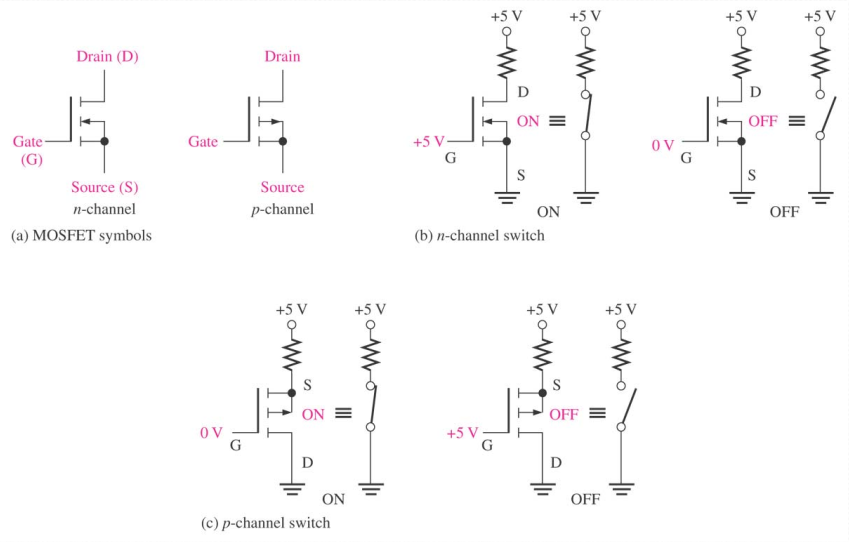
\includegraphics[width=0.8\linewidth]{fig/cmos.PNG}
	\caption{CMOS电路:\large\textbf{$n$内高,$p$外低}}
\end{figure}
\begin{figure}[htbp]
	\centering
	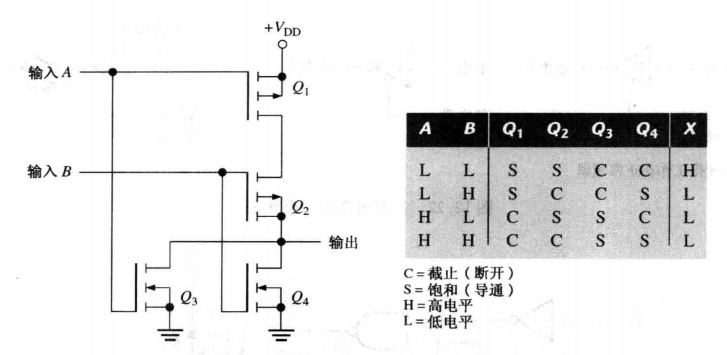
\includegraphics[width=0.6\linewidth]{fig/cmos_ex.PNG}
	\caption{CMOS或非门}
\end{figure}
\begin{figure}[htbp]
	\centering
	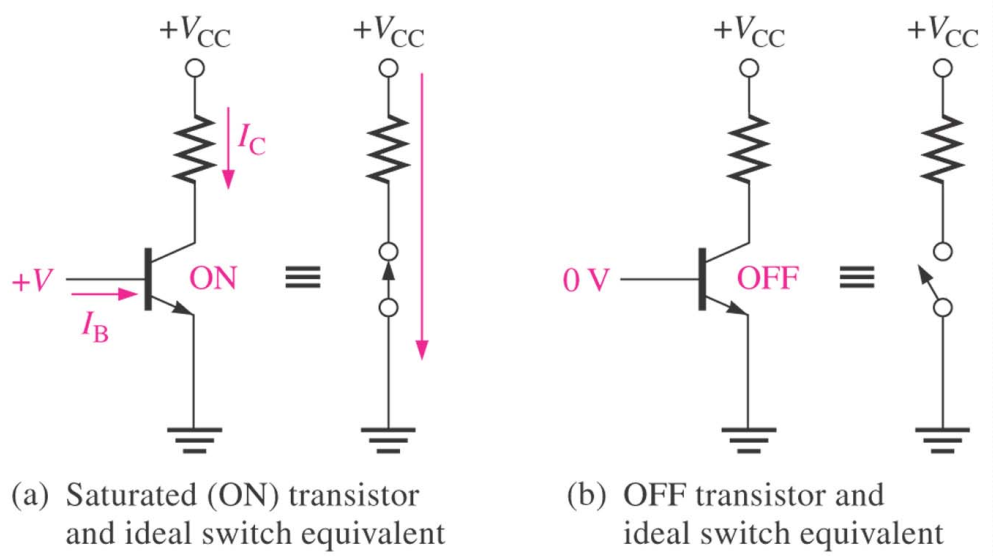
\includegraphics[width=0.6\linewidth]{fig/ttl.PNG}
	\caption{TTL电路}
\end{figure}
\begin{figure}[htbp]
\label{ttl_inverse}
	\centering
	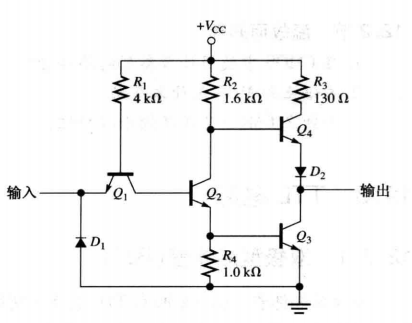
\includegraphics[width=0.6\linewidth]{fig/ttl_ex.PNG}
	\caption{TTL反相器}
\end{figure}
\par 由图\ref{ttl_inverse},$Q_1$被$V_{CC}$上拉,始终导通. 若输入为高电平,$Q_2$导通,$Q_3$导通,输出被下拉为低电平. 同时,$Q_2$在集电极处足够低的电压可以使$Q_4$截至.
\begin{figure}[htbp]
	\centering
	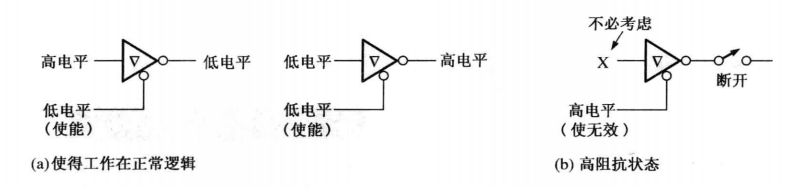
\includegraphics[width=0.6\linewidth]{fig/three_gates.PNG}
	\caption{三态门}
\end{figure}
\section{组合电路}
\subsection{基本逻辑门}
\begin{figure}[htbp]
	\centering
	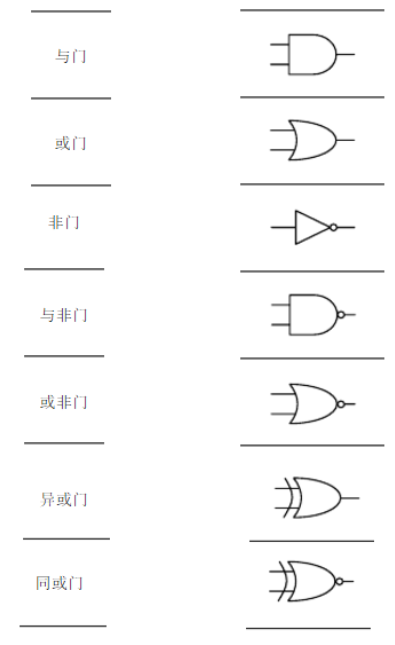
\includegraphics[width=0.6\linewidth]{fig/logic_gates.PNG}
	\caption{基本逻辑门}
\end{figure}
\subsection{布尔(Boolen)代数}
满足交换律、结合律、分配律
\[\begin{aligned}
A\ol{A}&=0 \qquad &A+\ol{A}&=1\\
A\ol{B}+\ol{A}B&=A\oplus B \qquad &AB+\ol{A}\ol{B}&=A\odot B
\end{aligned}\]
\[\begin{aligned}
A+BC&=A(1+B+C)+BC \qquad &A+\ol{A}B&=A(1+B)+\ol{A}B\\
&=(A+B)(A+C)\qquad & &=A+B
\end{aligned}\]

\subsection{卡诺(Karnaugh)图}
\begin{figure}[htbp]
	\centering
	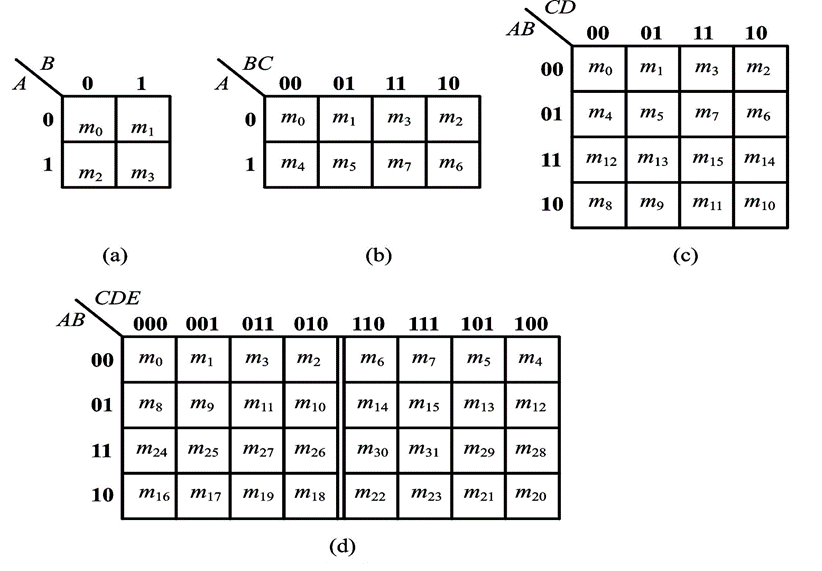
\includegraphics[width=0.8\linewidth]{fig/Karnaugh_graph.png}
	\caption{不同阶卡诺图}
\end{figure}
\begin{figure}[htbp]
	\centering
	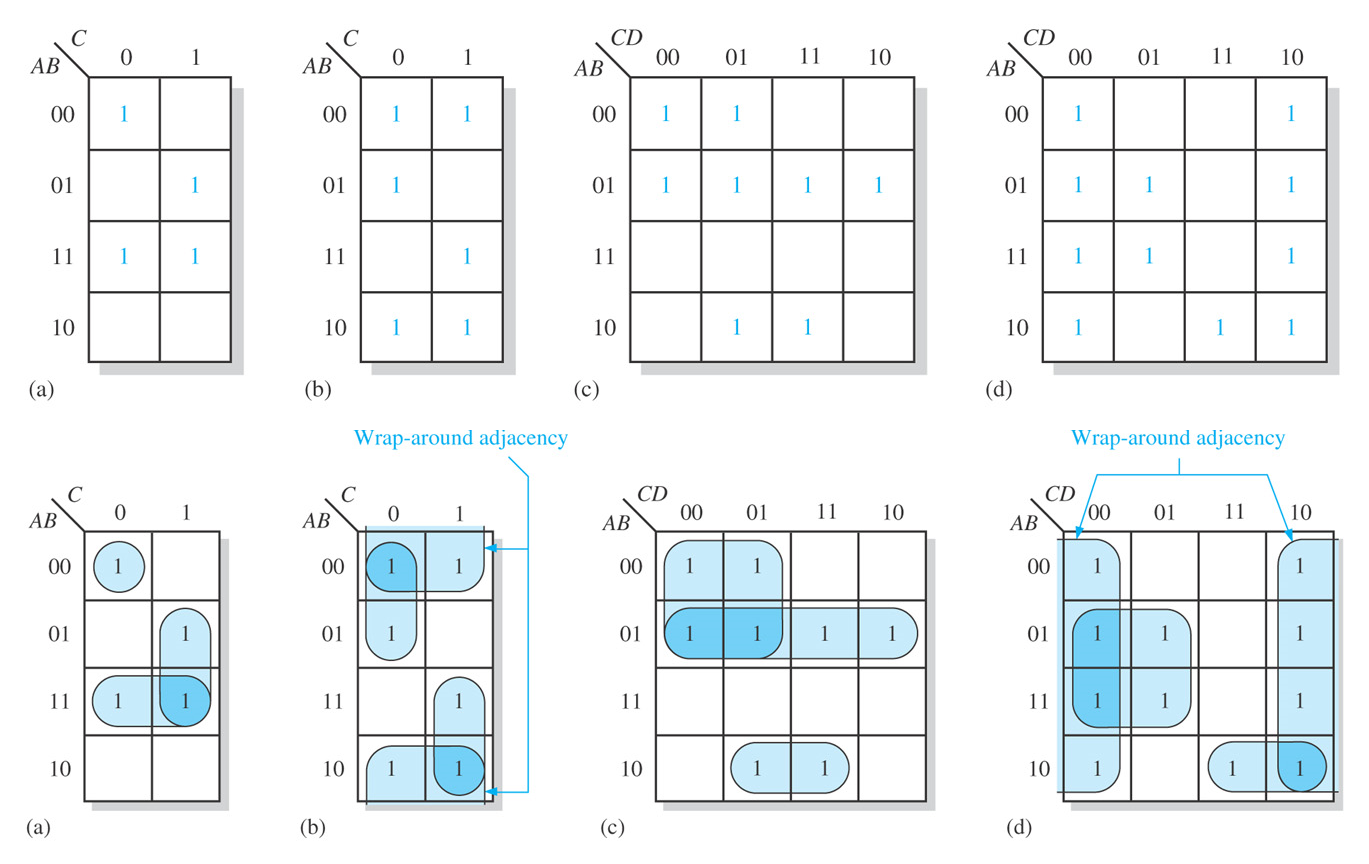
\includegraphics[width=0.8\linewidth]{fig/Karnaugh_example.png}
	\caption{Sum of Product(SOP)化简}
\end{figure}

\subsection{功能器件}
\subsubsection{加法器}
\begin{figure}[htbp]
	\centering
	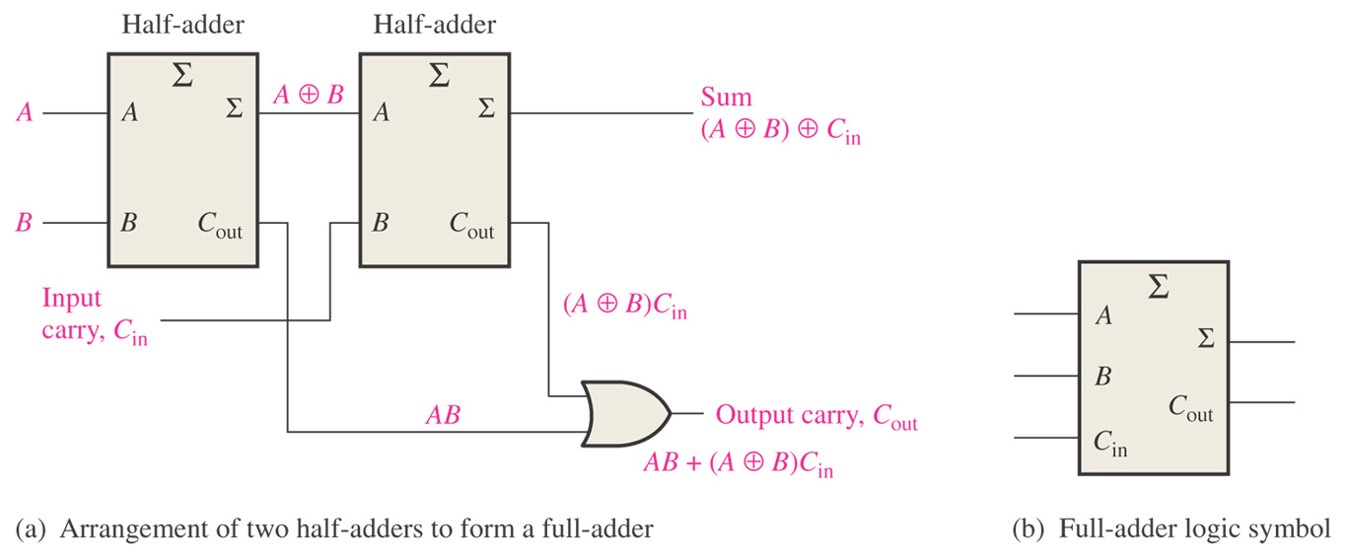
\includegraphics[width=0.8\linewidth]{fig/adder.jpg}
	\caption{半加法器与全加法器}
\end{figure}
\begin{figure}[htbp]
	\centering
	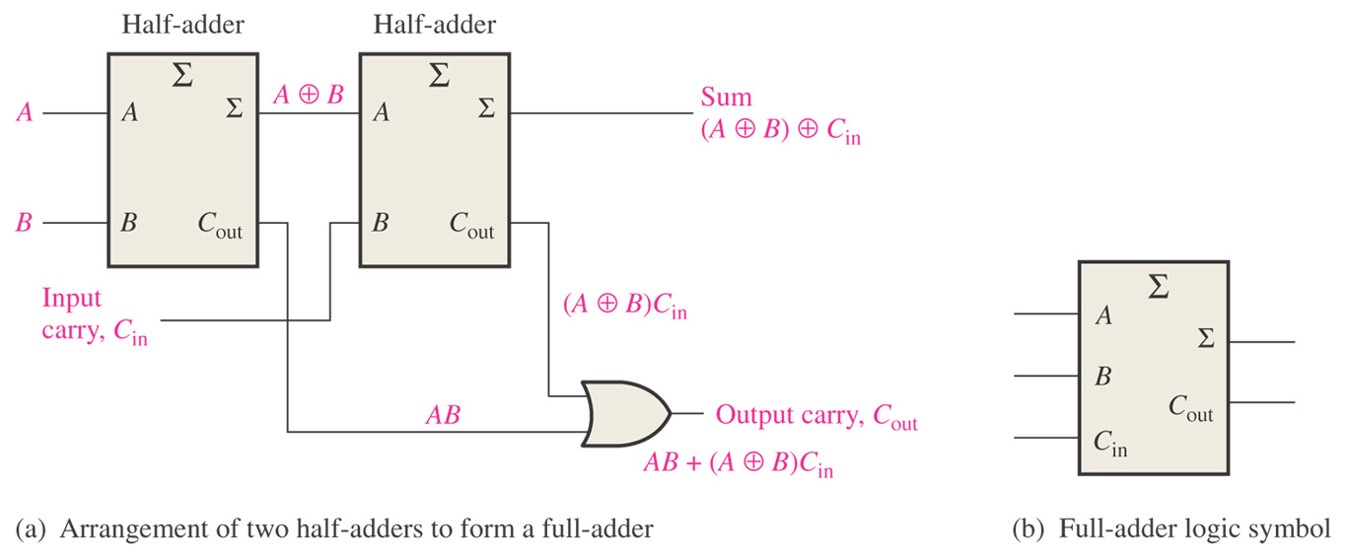
\includegraphics[width=0.8\linewidth]{fig/adder.jpg}
	\caption{异步加法器改造为同步加法器}
\end{figure}
\[\begin{aligned}
&\text{Carry generation: }&C_g&=AB\\
&\text{Carry propagation: }&C_g&=AB\\
&\text{Output carry: }&C_g&=AB\\
& &C_{in2}&=C_{out1}=C_{g1}+C_{p1}C_{in1}\\
& &C_{in3}&=C_{out2}=C_{g2}+C_{p2}C_{in2}=C_{g2}+C_{p2}(C_{g1}+C_{p1}C_{in1})
\end{aligned}\]
\subsubsection{比较器(Comparator)}
\begin{figure}[htbp]
	\centering
	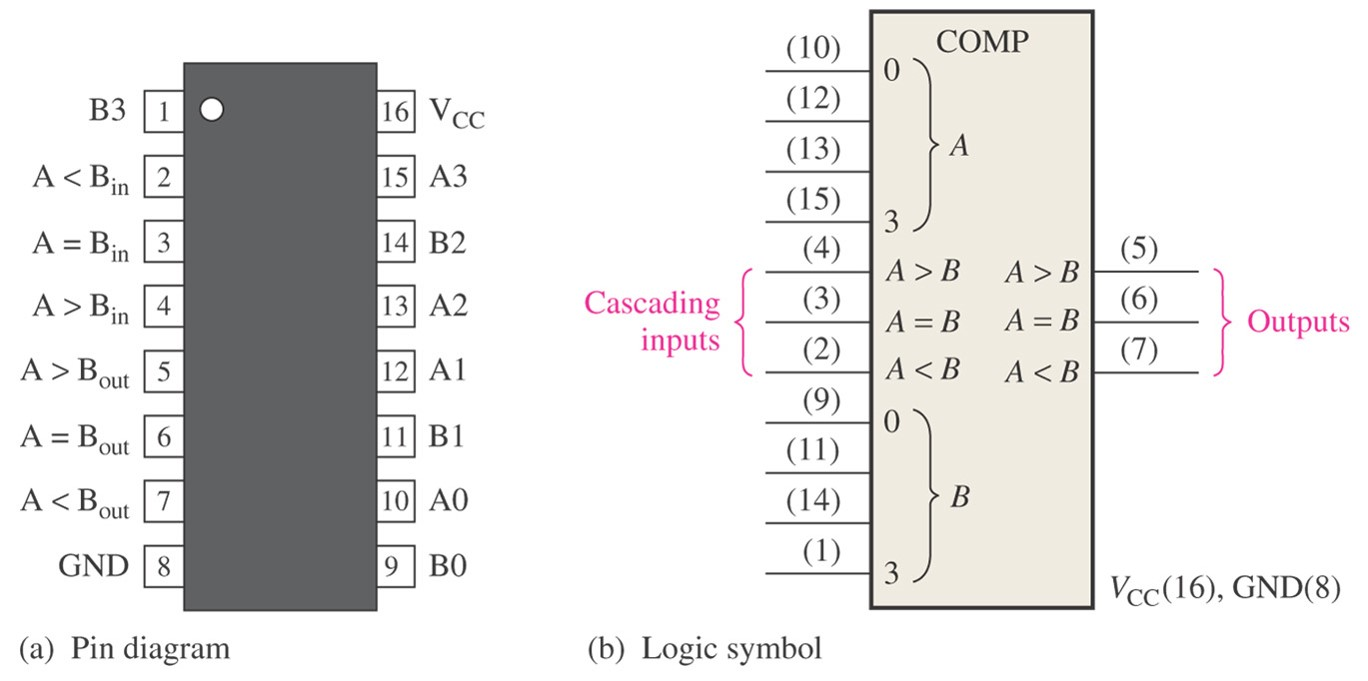
\includegraphics[width=0.8\linewidth]{fig/comparator.jpg}
	\caption{比较器}
\end{figure}
\subsubsection{译码器(Decoder)}
BCD码转对应端口输出,注意输出是反的
\begin{figure}[htbp]
	\centering
	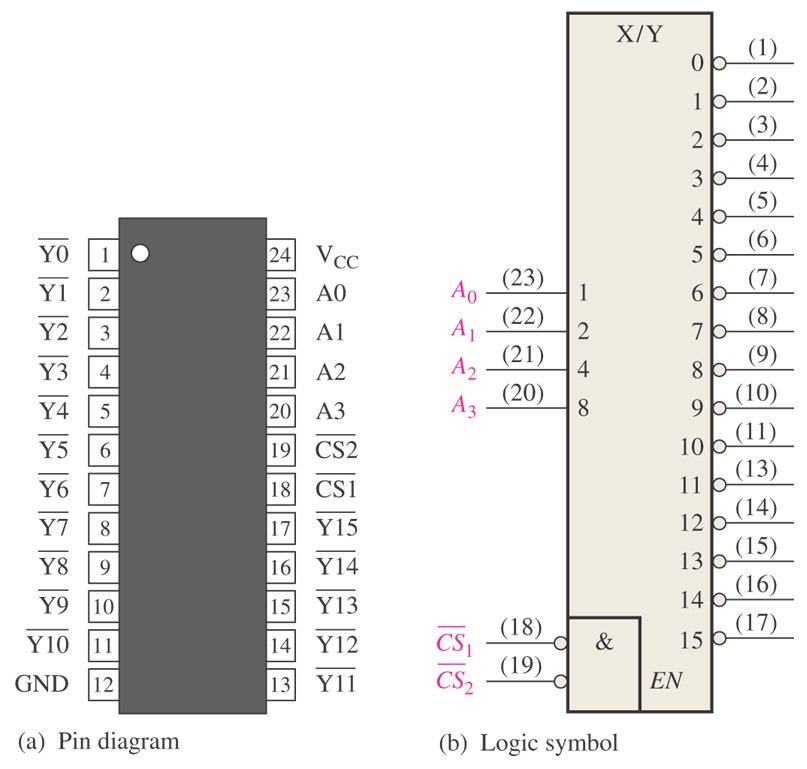
\includegraphics[width=0.5\linewidth]{fig/decoder.jpg}
	\caption{译码器}
\end{figure}
\par BCD转7段数码管
\begin{enumerate}
	\item 共阴(cathode):高电平亮
	\item 共阳(anode):低电平亮
\end{enumerate}
\subsubsection{编码器(Encoder)}
输入转BCD码
\begin{figure}[htbp]
	\centering
	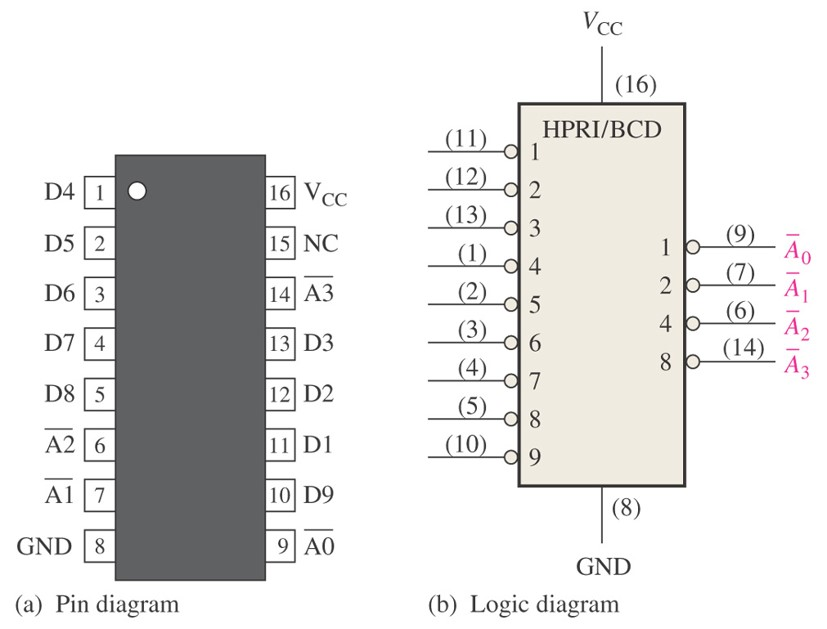
\includegraphics[width=0.6\linewidth]{fig/encoder.jpg}
	\caption{编码器}
\end{figure}
\subsubsection{选择器(Multiplexer)}
通过BCD码选择对应路输出
\begin{figure}[htbp]
	\centering
	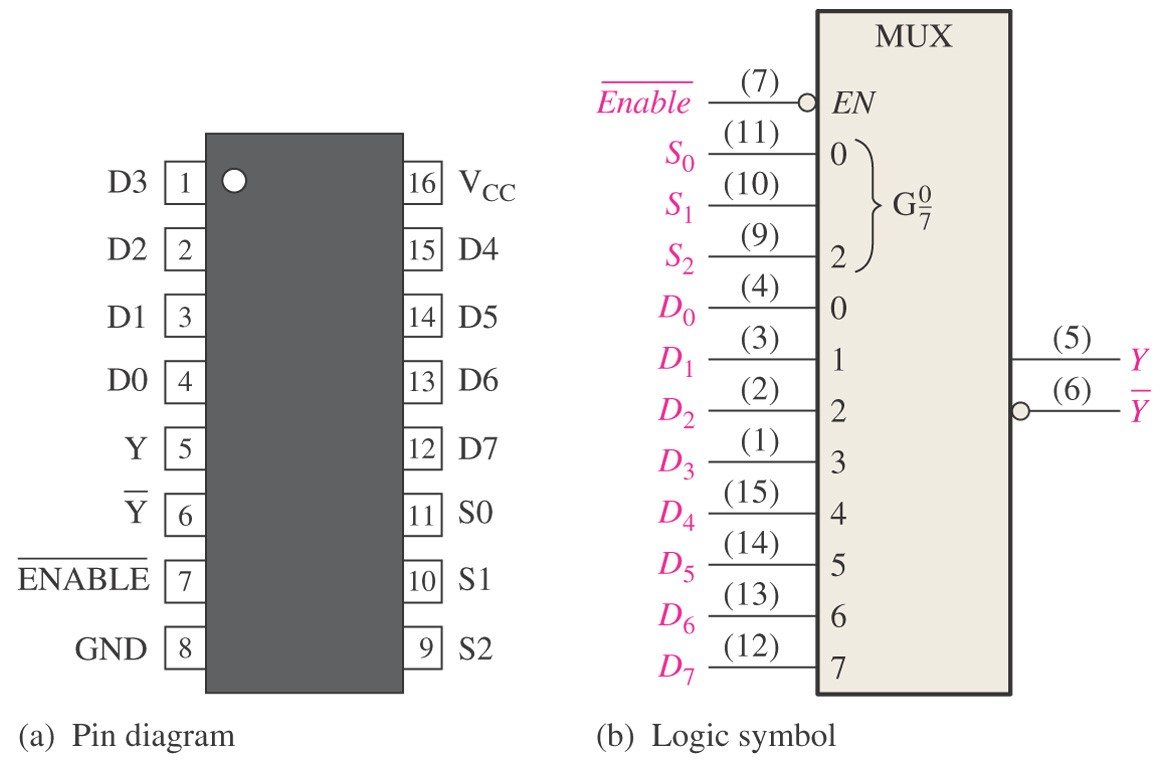
\includegraphics[width=0.6\linewidth]{fig/multiplexer.jpg}
	\caption{选择器}
\end{figure}
\subsubsection{多路分配器(Demultiplexer)}
将对应输入分配到对应输出路

\subsection{竞争与冒险}
\begin{enumerate}
	\item 竞争(race):输入到输出途径不同,延时时间不同,到达输出的时间不同
	\item 冒险(hazard):竞争结果导致逻辑电路产生错误输出
\end{enumerate}
\par 如$F=AB+\ol{A}C$,因为取非,导致两条道路时间不同,使得输出出现毛刺现象
\par 可加入冗余项以避免冒险,如改成$F=AB+\ol{A}C+BC$
\section{时序电路}
\subsection{锁存器}
\par 用于存储数据
\begin{figure}[htbp]
	\centering
	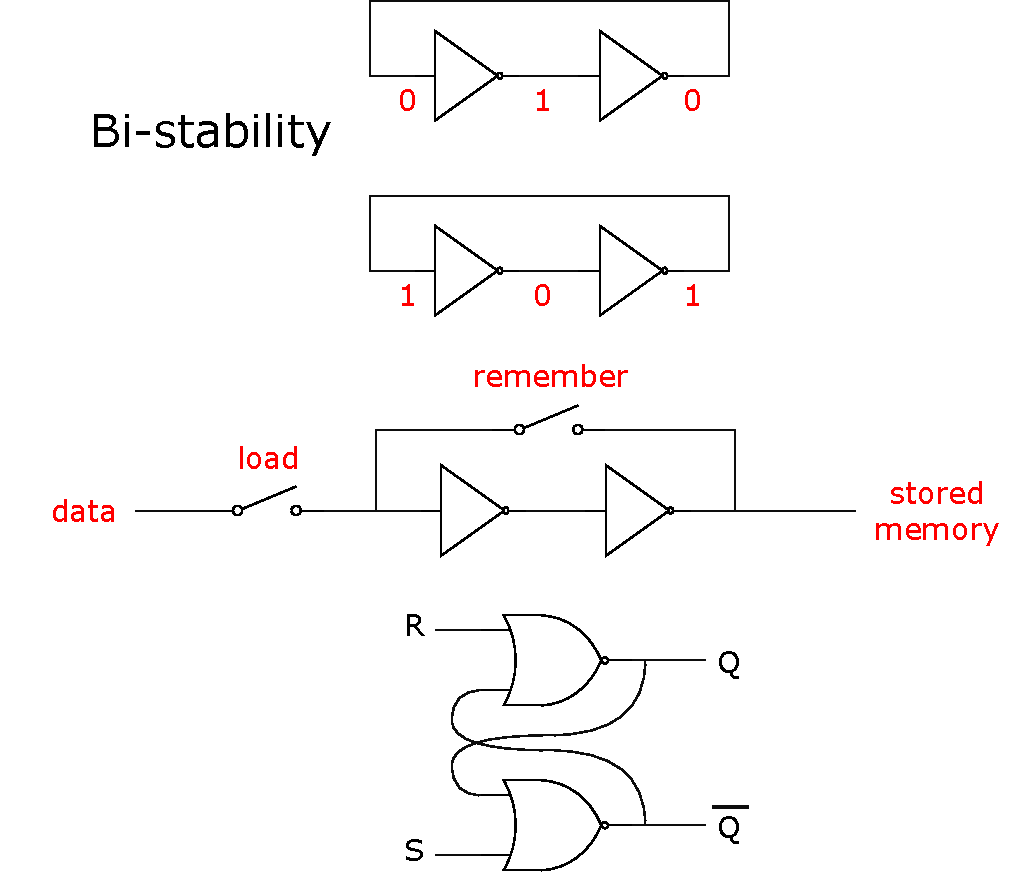
\includegraphics[width=0.6\linewidth]{fig/latches.pdf}
	\caption{SR锁存器(latch)}
\end{figure}
\par SR锁存器状态表
\begin{center}
\begin{tabular}{|c|c|c|c|}
\hline
S & R & 状态\\\hline
0 & 0 & 不变\\\hline
0 & 1 & 复位\\\hline
1 & 0 & 置位\\\hline
1 & 1 & N/A\\\hline
\end{tabular}
\end{center}
\par D锁存器状态:0复位,1置位
\par 门(选通端):决定是否运作

\subsection{触发器}
\subsubsection{SR/D触发器}
\par 触发器状态变化与锁存器相同
\begin{figure}[htbp]
	\centering
	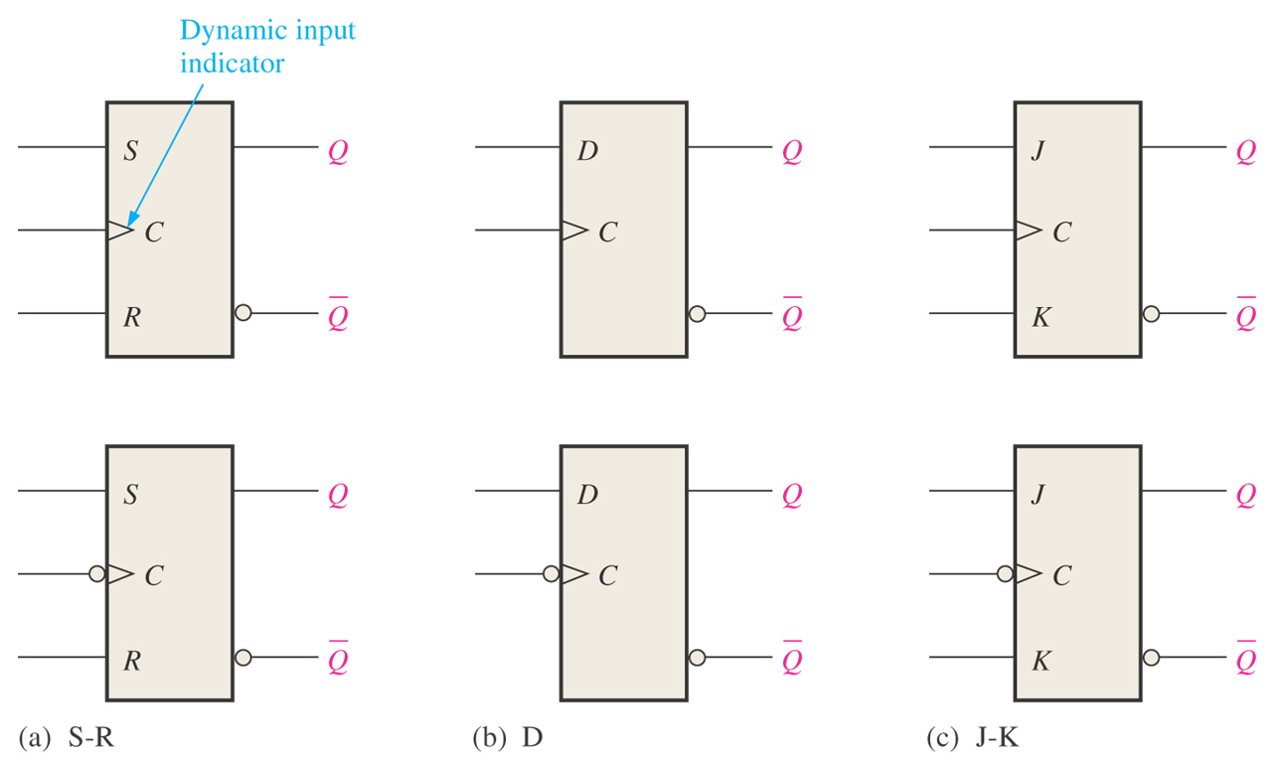
\includegraphics[width=0.6\linewidth]{fig/flip-flops.png}
	\caption{触发器}
\end{figure}
边缘触发其实通过竞争实现(如输入加一个与门后与非$\ol{A\ol{A}}$)
\subsubsection{JK触发器}
\begin{figure}[htbp]
	\centering
	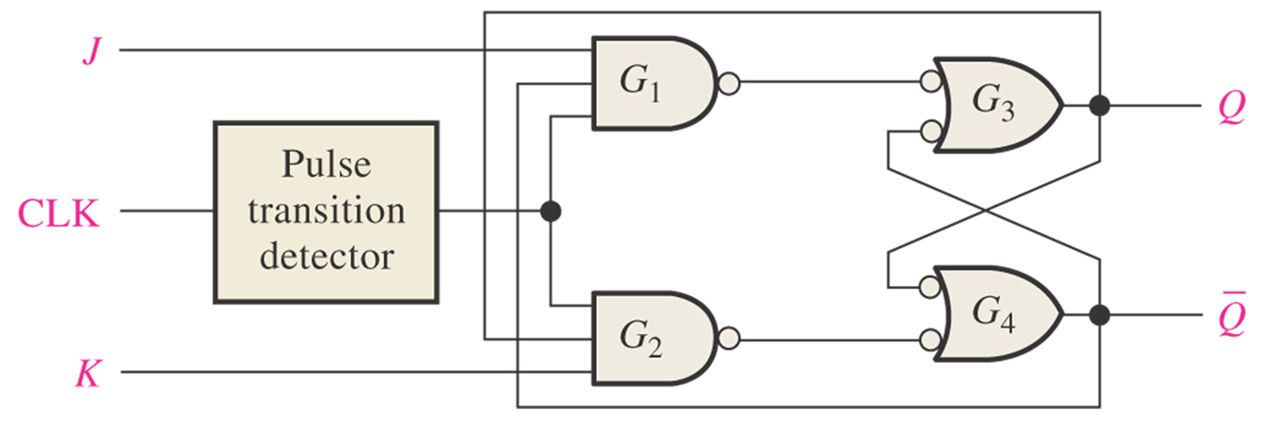
\includegraphics[width=0.6\linewidth]{fig/JK_flip-flop.png}
	\caption{JK触发器}
\end{figure}
\par JK触发器状态表
\begin{center}
\begin{tabular}{|c|c|c|c|}
\hline
J & K & 状态\\\hline
0 & 0 & 不变\\\hline
0 & 1 & 复位\\\hline
1 & 0 & 置位\\\hline
1 & 1 & 转换\\\hline
\end{tabular}
\end{center}
\par 注意看有无\textcolor{red}{bubble},看是上升沿还是下降沿
\subsubsection{应用}
\begin{enumerate}
	\item 并行数据传输:接同一时钟
	\item 分频:JK均接高,遇上升沿才触发,故可实现
\begin{figure}[htbp]
	\centering
	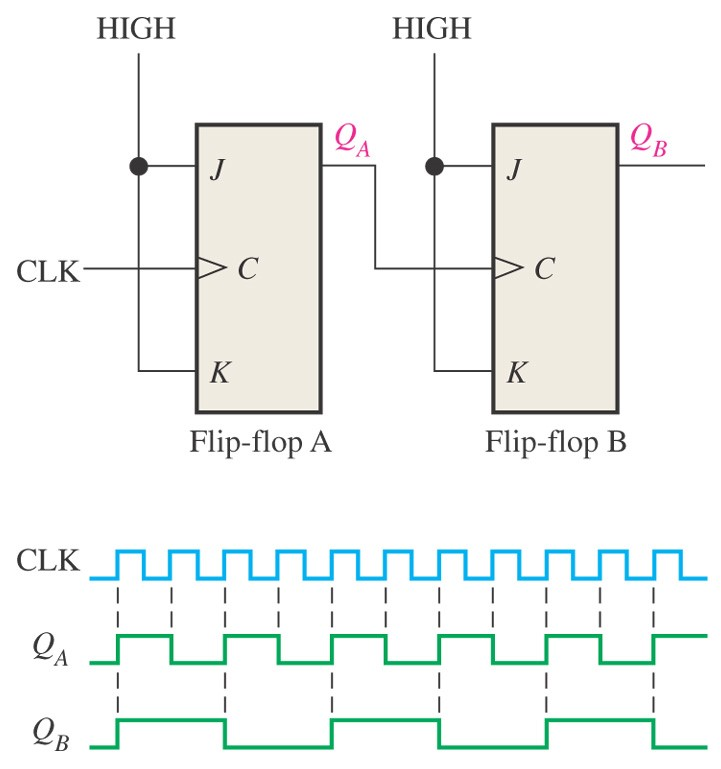
\includegraphics[width=0.4\linewidth]{fig/frequency_divisor.jpg}
	\caption{分频器}
\end{figure}
	\item 计数器:也相当于分频
\begin{figure}[htbp]
	\centering
	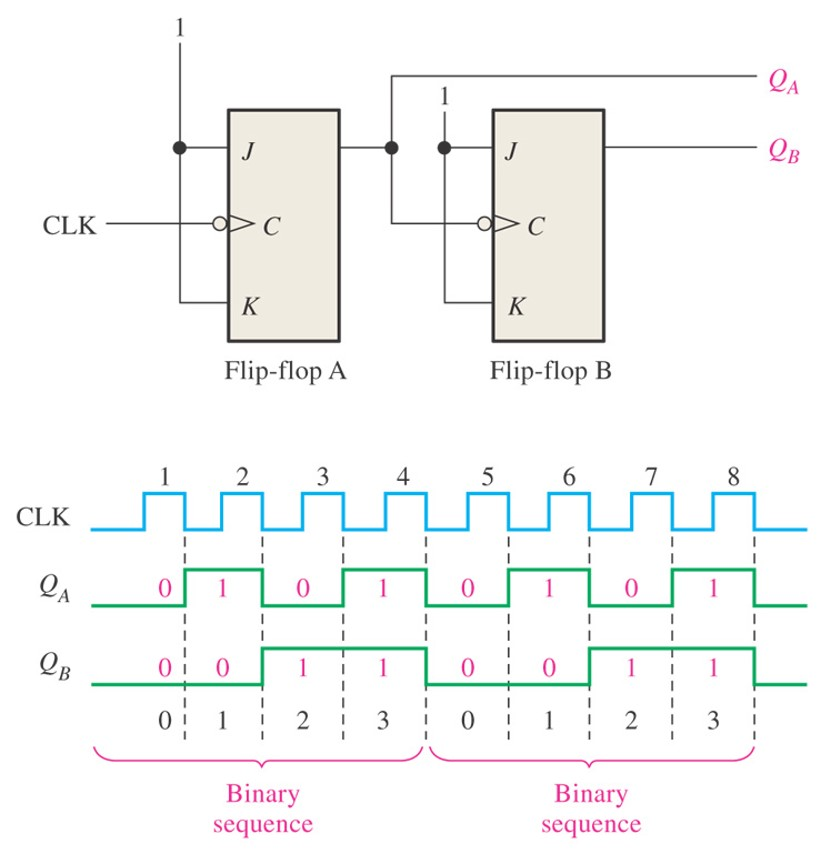
\includegraphics[width=0.4\linewidth]{fig/counter.jpg}
	\caption{计数器}
\end{figure}
\end{enumerate}

\subsection{单稳态触发器}
\begin{figure}[htbp]
	\centering
	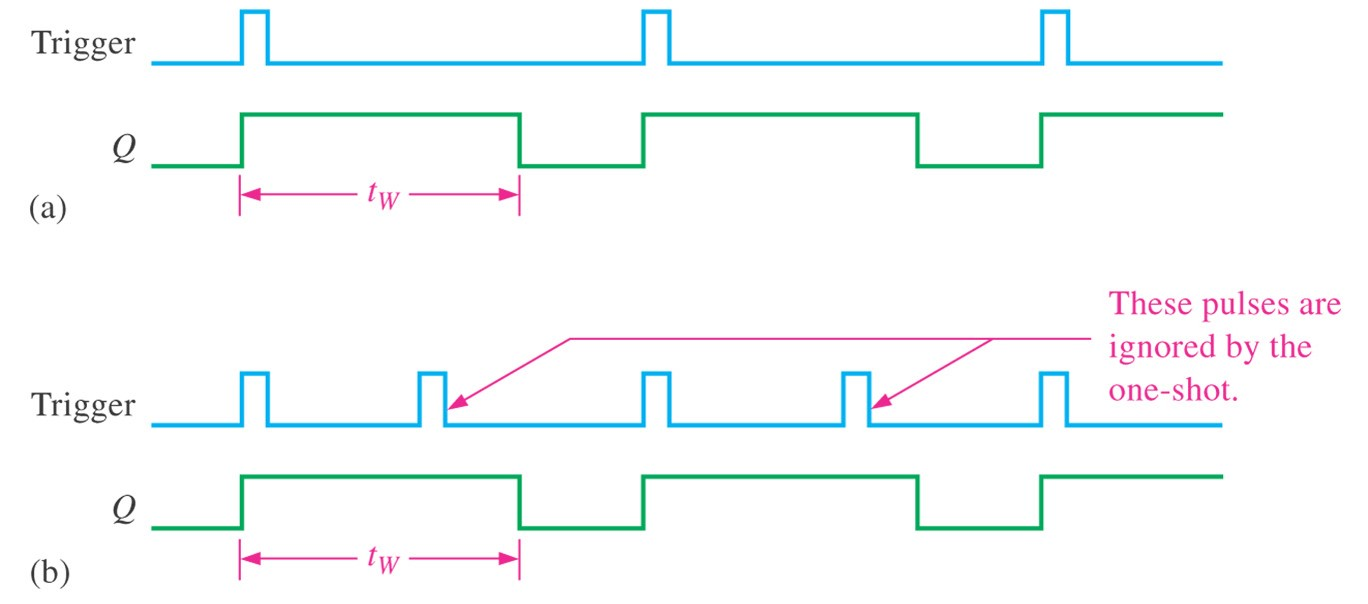
\includegraphics[width=0.6\linewidth]{fig/one-shot.jpg}
	\caption{单稳态触发器(不可重复触发)}
\end{figure}

\subsection{555计时器}
\begin{itemize}
	\item 单稳态触发器(mono-stable one-shot)
	\item 非稳态多谐振荡器(astable multi-vibration oscillator)
\end{itemize}
\begin{figure}[htbp]
	\centering
	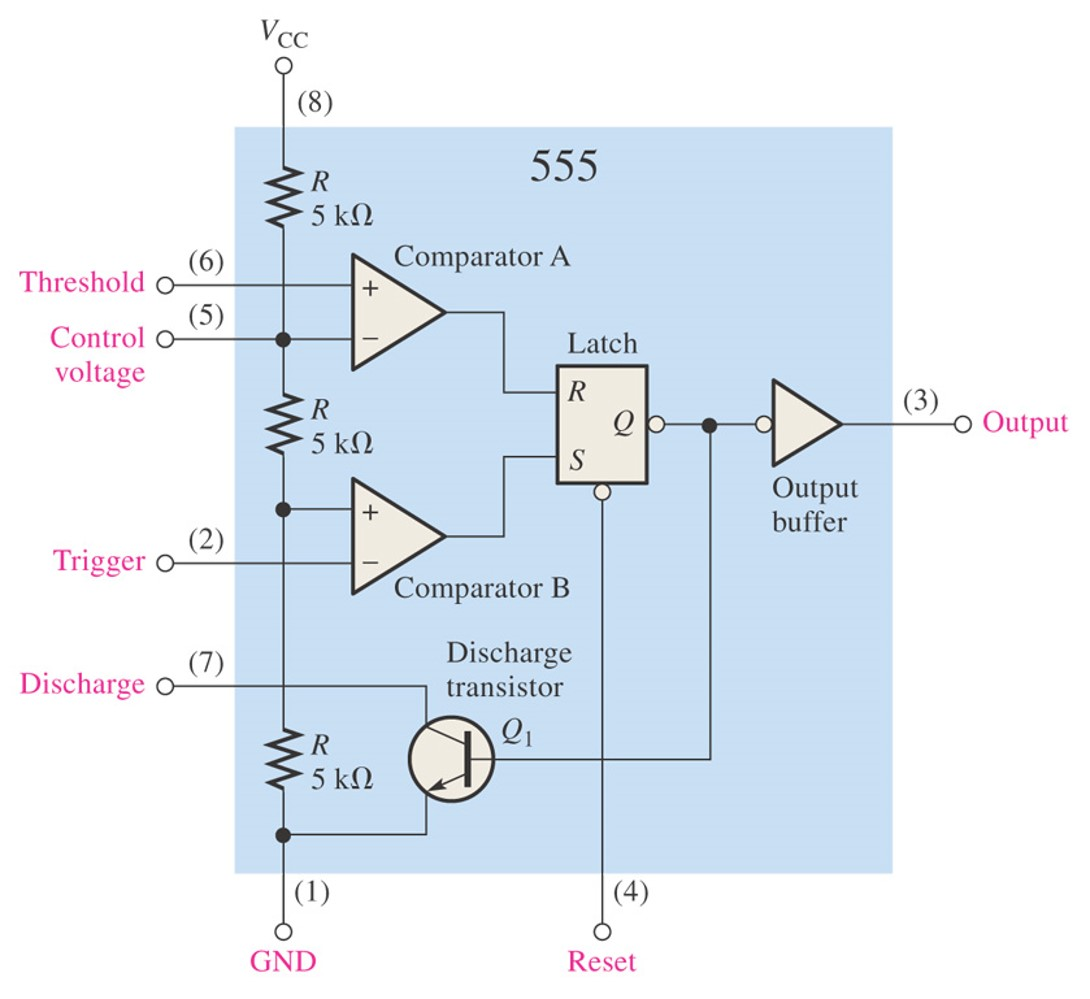
\includegraphics[width=0.6\linewidth]{fig/555timer.jpg}
	\caption{555计时器}
\end{figure}
\[f=\dfrac{1.44}{(R_1+2R_2)C_1}\]
\[DC=\dfrac{R_1+R_2}{R_1+2R_2}\times 100\%\]

\subsection{移位寄存器}
\subsubsection{约翰逊计数器}
\begin{figure}[htbp]
	\centering
	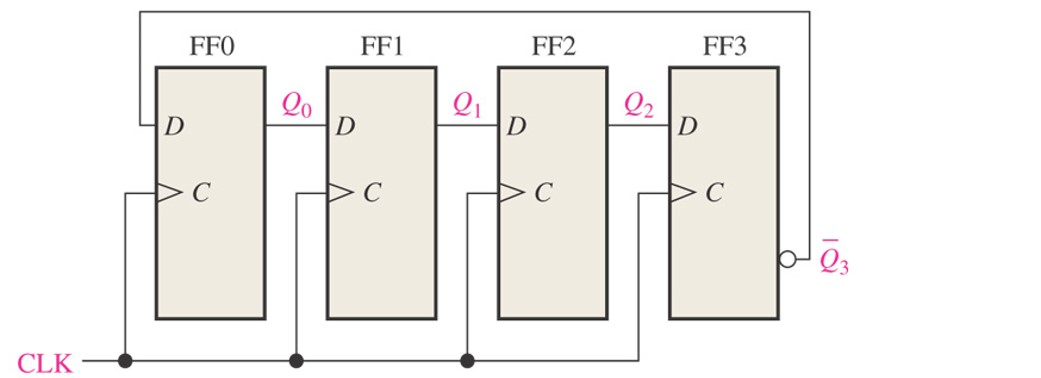
\includegraphics[width=0.6\linewidth]{fig/johnson.jpg}
	\caption{约翰逊(Johnson)计数器}
\end{figure}
\par 计数范围$M=2N$
\begin{center}
\begin{tabular}{|c|c|c|c|c|}
\hline
计数 & $Q_0$ & $Q_1$ & $Q_2$ & $Q_3$\\\hline
0 & 0 & 0 & 0 & 0\\\hline
1 & 1 & 0 & 0 & 0\\\hline
2 & 1 & 1 & 0 & 0\\\hline
3 & 1 & 1 & 1 & 0\\\hline
4 & 1 & 1 & 1 & 1\\\hline
5 & 0 & 1 & 1 & 1\\\hline
6 & 0 & 0 & 1 & 1\\\hline
7 & 0 & 0 & 0 & 1\\\hline
\end{tabular}
\end{center}
\subsubsection{环计数器}
\par 计数范围$M=N$
\begin{figure}[htbp]
	\centering
	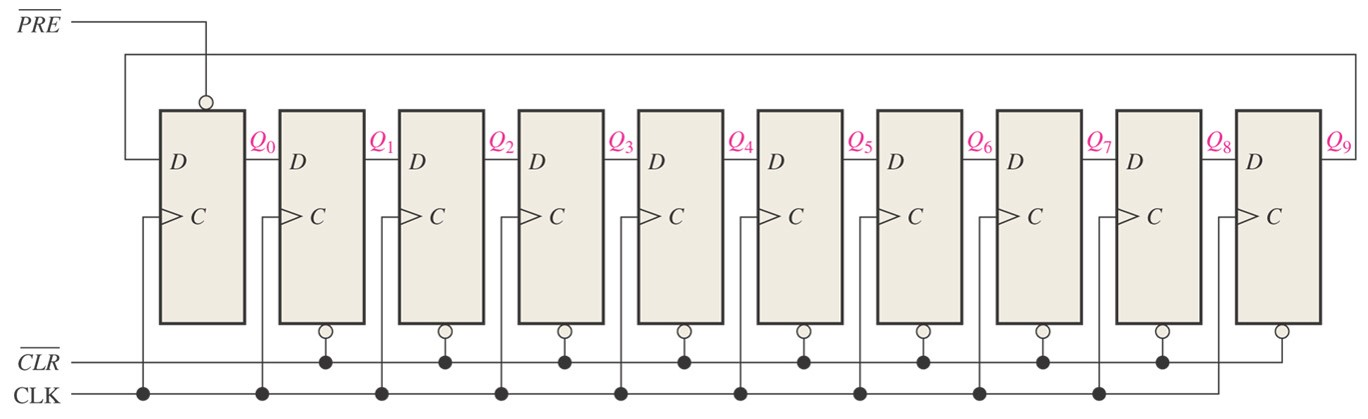
\includegraphics[width=0.6\linewidth]{fig/ring_counter.jpg}
	\caption{环计数器}
\end{figure}
\par 初始置为$1000000000$

\subsection{计数器}
\subsubsection{同步异步计数器}
\begin{figure}[htbp]
	\centering
	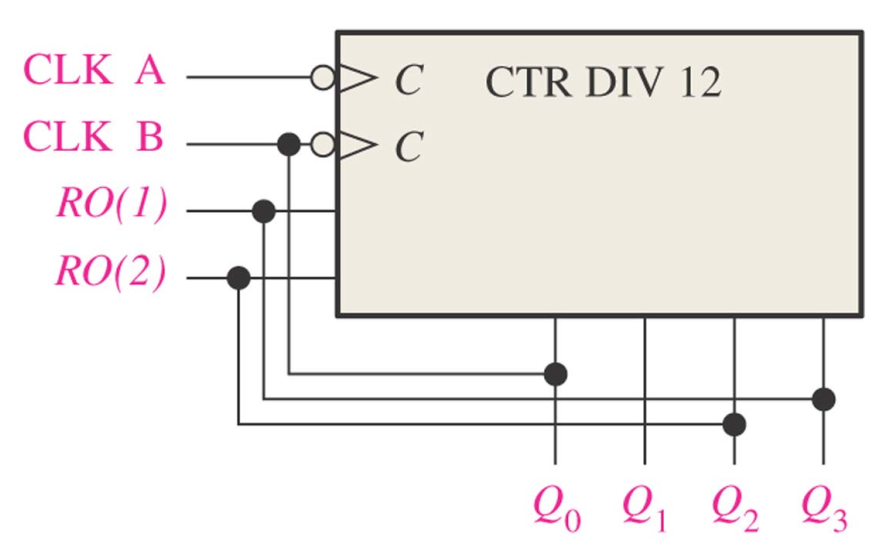
\includegraphics[width=0.3\linewidth]{fig/74ls93.PNG}
	\caption{16进制计数器}
\end{figure}
\par RO(1)与RO(2)同时为高时清零,CLK A控制二进制计数器($Q_0$),CLK B控制八进制计数器($Q_1\thicksim Q_3$),故将$Q_0$输出与八进制计数器相连可得十六进制计数器
\begin{figure}[htbp]
	\centering
	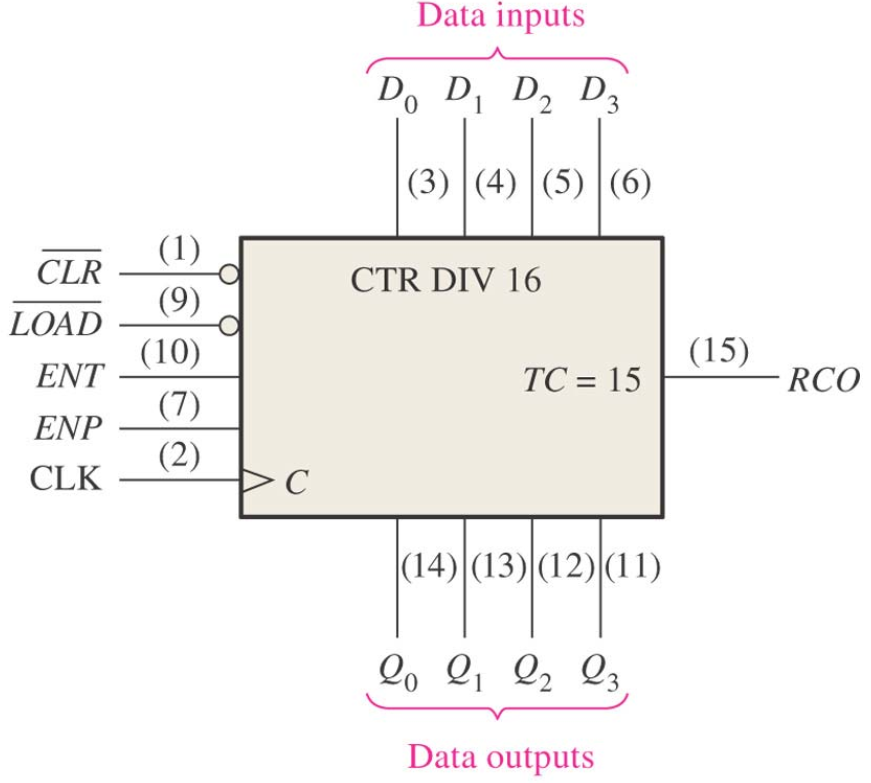
\includegraphics[width=0.3\linewidth]{fig/74hc163.PNG}
	\caption{4位同步二进制计数器}
\end{figure}
\par $\ol{LOAD}$为低时读取数据,ENT、ENP为使能端,同时高电平有效,RCO为进位端
\subsubsection{应用}
\begin{figure}[htbp]
	\centering
	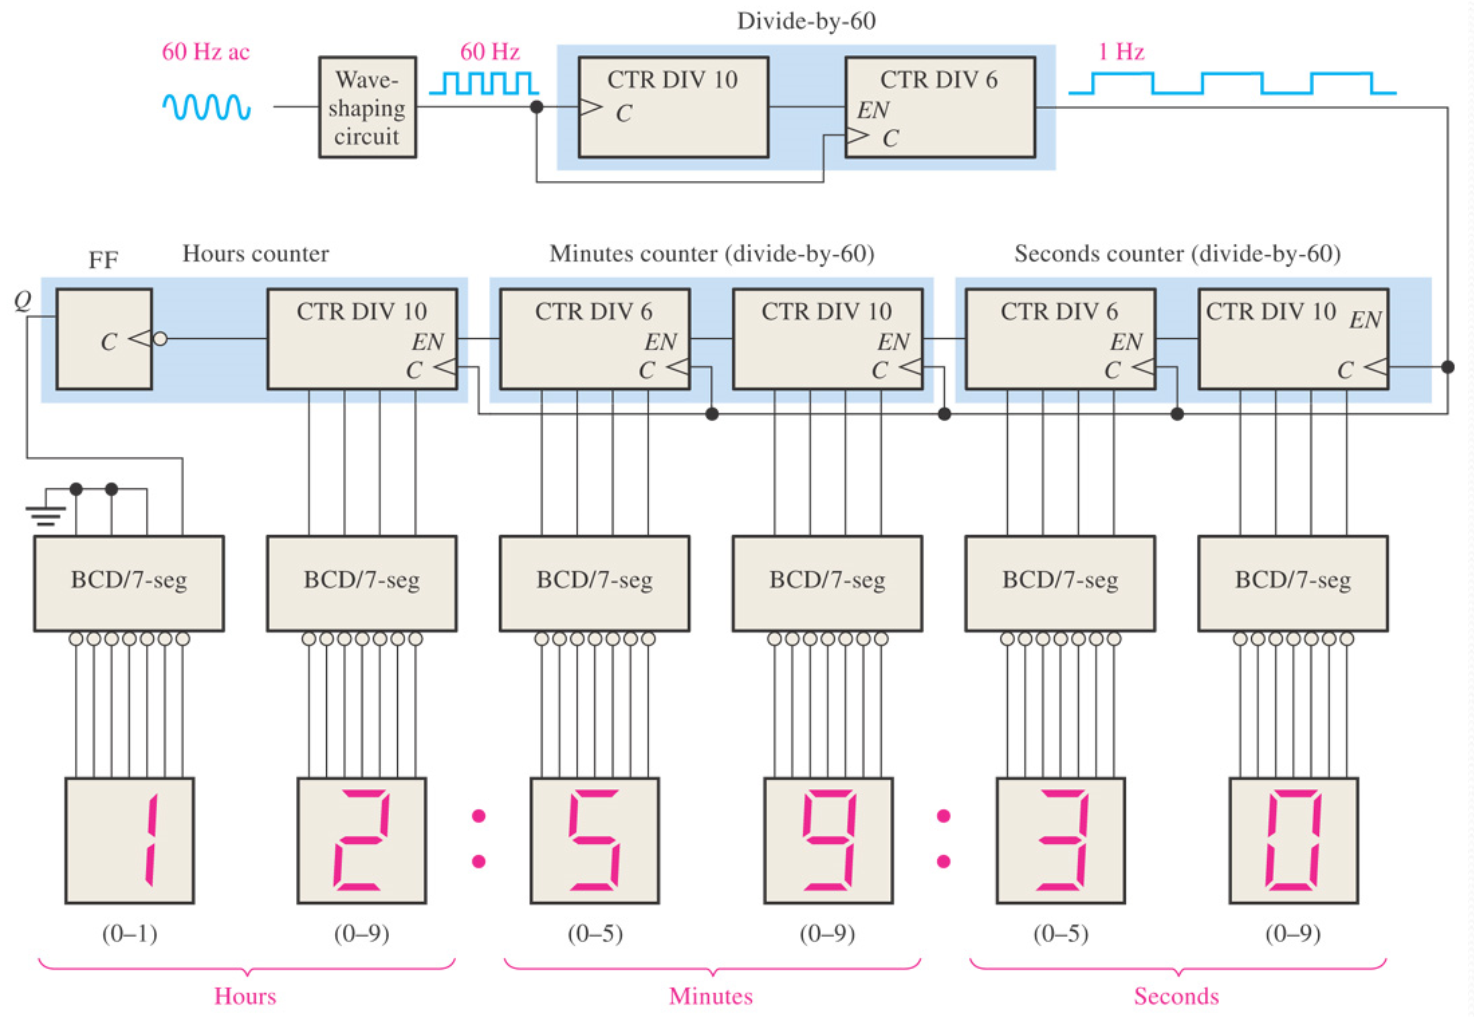
\includegraphics[width=0.6\linewidth]{fig/timer.PNG}
	\caption{时钟}
\end{figure}
\section{电路设计}
\subsection{电路分类}
\begin{enumerate}
\item 摩尔(Moore)电路
\begin{figure}[htbp]
	\centering
	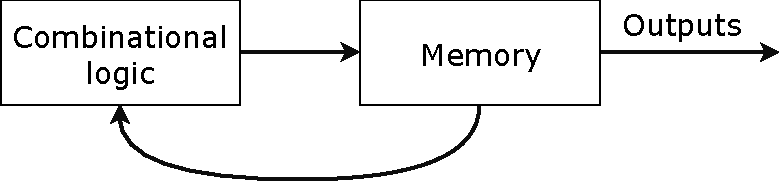
\includegraphics[width=0.4\linewidth]{fig/moore_machine.pdf}
	\caption{触发器}
\end{figure}
\item 米勒(Mealy)电路
\begin{figure}[htbp]
	\centering
	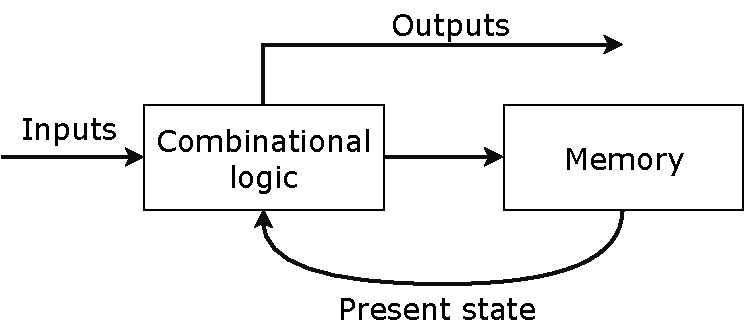
\includegraphics[width=0.4\linewidth]{fig/mealy_machine.pdf}
	\caption{触发器}
\end{figure}
\end{enumerate}
\subsection{设计步骤}
\par 基于状态转移表格的方法
\begin{enumerate}
    \item 状态图
    \item 次态表
    \item 触发器转移表
\begin{center}
\begin{tabular}{|c|c|c|c|}
\hline
$Q^n$ & $Q^{n+1}$ & J & K\\\hline
0 & 0 & 0 & X\\\hline
0 & 1 & 1 & X\\\hline
1 & 0 & X & 1\\\hline
1 & 1 & X & 0\\\hline
\end{tabular}
\end{center}
    \item 触发器JK卡诺图
    \item JK驱动方程
    \item 时序电路
\end{enumerate}
\par 基于状态方程的方法
\begin{enumerate}
	\item 状态表
	\item 次态卡诺图
	\item 状态方程 $Q^{n+1}=J\ol{Q^n}+\ol{K}Q^n$
	\item 驱动方程
	\item 时序电路
\end{enumerate}
\subsection{实例操作}
\par 目的:用JK触发器实现一个12进制同步计数器
\begin{enumerate}
    \item 状态转换图
    \begin{figure}[H]
        \centering
        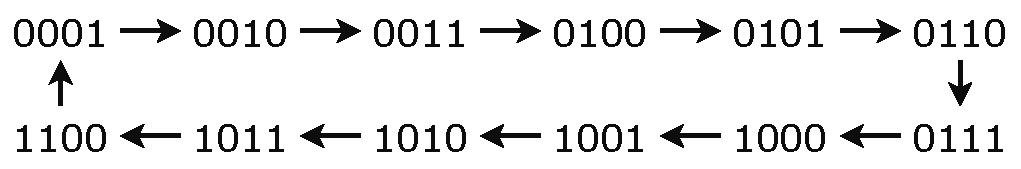
\includegraphics[width=0.7\linewidth]{fig/12system_state.pdf}
    \end{figure}
    \item 确定电路所需触发器数目\\
    由于$2^4=16>12$,故需要$4$个JK触发器
    \item 次态卡诺图
    \begin{figure}[H]
        \centering
        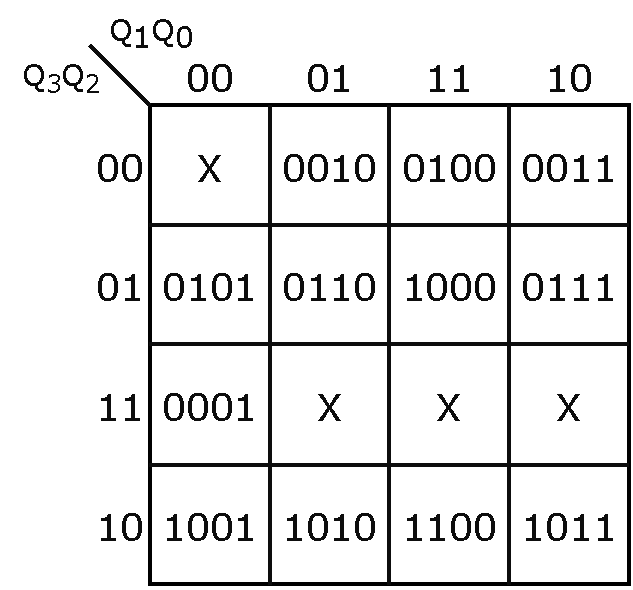
\includegraphics[width=0.4\linewidth]{fig/Karnaugh_12system.pdf}
    \end{figure}
    \item 触发器状态方程,由卡诺图可得
    \[\begin{aligned}
    Q_0^{n+1}&=\overline{Q_0}\\
    Q_1^{n+1}&=Q_0\overline{Q_1}+\overline{Q_0}Q_1\\
    Q_2^{n+1}&=Q_0Q_1\ol{Q_2}+\ol{Q_1}Q_2\ol{Q_3}+\ol{Q_0}Q_2\ol{Q_3}\\
    Q_3^{n+1}&=\ol{Q_2}Q_3+Q_0Q_1Q_2\ol{Q_3}
    \end{aligned}\]
    \item 触发器驱动方程,由
    \[Q^{n+1}=J\ol{Q^n}+\ol{K}Q^n\]
    将状态方程整理为上式形式,可得
    \[\begin{aligned}
    J_0&=1 \qquad &K_0&=1\\
    J_1&=Q_0 \qquad &K_0&=Q_0\\
    J_2&=Q_1Q_0 \qquad &K_2&=\ol{\ol{Q_3}\ol{Q_1}+\ol{Q_3}\ol{Q_0}}=\ol{Q_3}+Q_1Q_0\\
    J_3&=Q_2Q_1Q_0 \qquad &K_3&=Q_2
    \end{aligned}\]
    \item 检查自启动\\
    当输入为1111和0000时,可自动跳转至0001;输入为1101时,跳转至0010;输入为1110时,跳转至0011
\end{enumerate}
\par Proteus电路图连接如下
\begin{figure}[H]
    \centering
    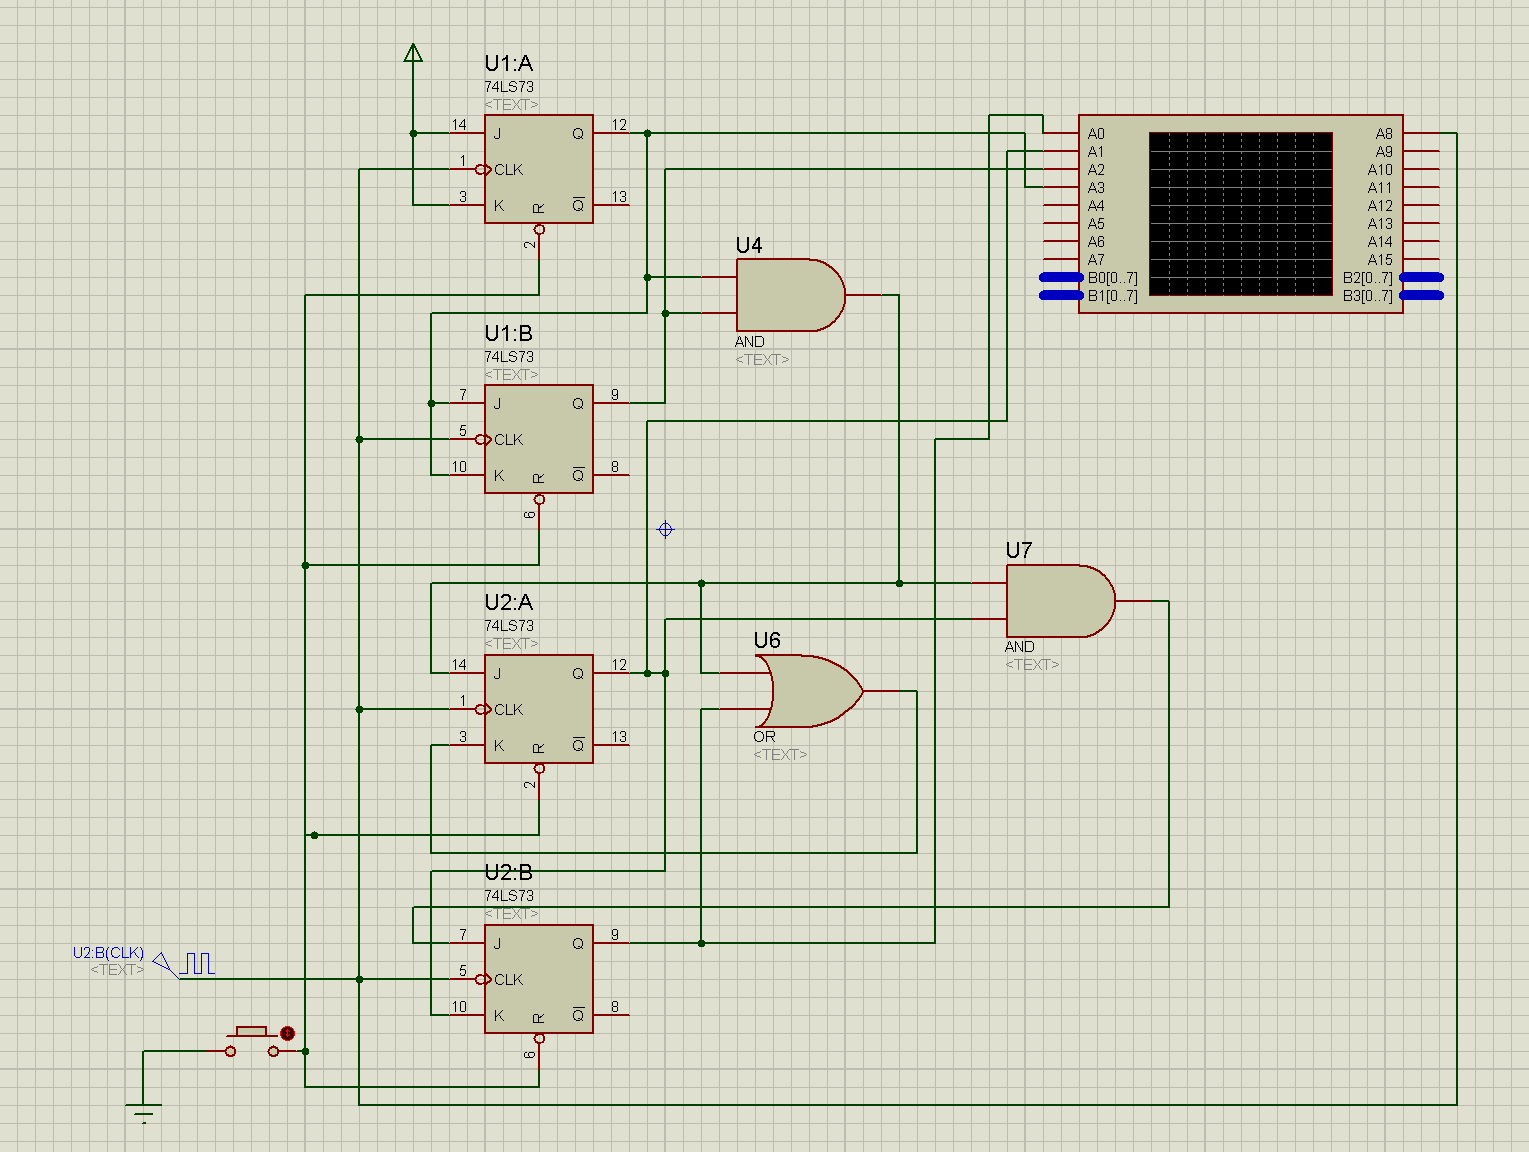
\includegraphics[width=0.9\linewidth]{fig/12system_protues.PNG}
\end{figure}
\par 仿真结果如下
\begin{figure}[H]
    \centering
    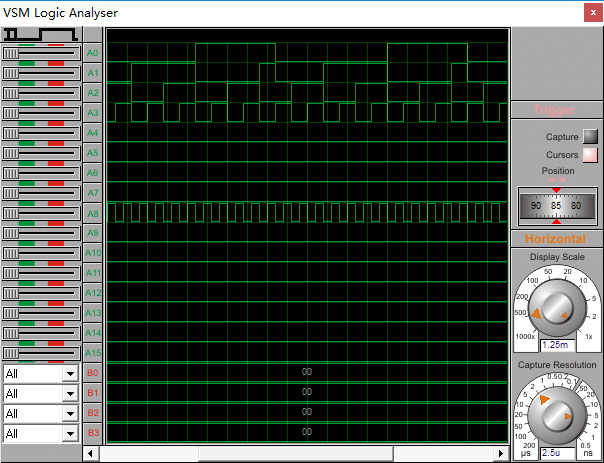
\includegraphics[width=0.6\linewidth]{fig/12system_wave.PNG}
\end{figure}

\end{document}